\documentclass{article}
\usepackage[a4paper,left=3cm,right=3cm,top=3cm,bottom=3cm]{geometry}
\usepackage[utf8]{inputenc}
\usepackage[T1]{fontenc}
\usepackage{latexsym,amsfonts,amsmath,amssymb,amstext,graphicx,titlesec,ae,aecompl,mathtools,tabularx, multirow, cancel, nicefrac,subcaption, blindtext, floatrow}
\setlength{\parindent}{0pt}
\newfloatcommand{capbtabbox}{table}[][\FBwidth]


\begin{document}

\begin{titlepage}
       \begin{center}
             \begin{huge}
				   %% Update assignment number here
                   \textbf{Assignment 4}
             \end{huge}
       \end{center}

       \begin{center}
             \begin{large}
                   Computational Intelligence, SS2020
             \end{large}
       \end{center}

       \begin{center}
 \begin{tabularx}{\textwidth}{|>{\hsize=.33\hsize}X|>{\hsize=.33\hsize}X|>{\hsize=.33\hsize}X|} 

                   \hline
                   \multicolumn{3}{|c|}{\textbf{Team Members}} \\
                   \hline
                   Last name & First name & Matriculation Number \\
                   \hline
                   Blöcher & Christian & 01573246 \\
                   \hline
                   Bürgener & Max & 01531577 \\
                   \hline
                    &  &  \\
                   \hline

             \end{tabularx}
       \end{center}
\end{titlepage}


\section{Linear SVM}

\subsection{Plots}

\begin{figure}[!ht]
\centering
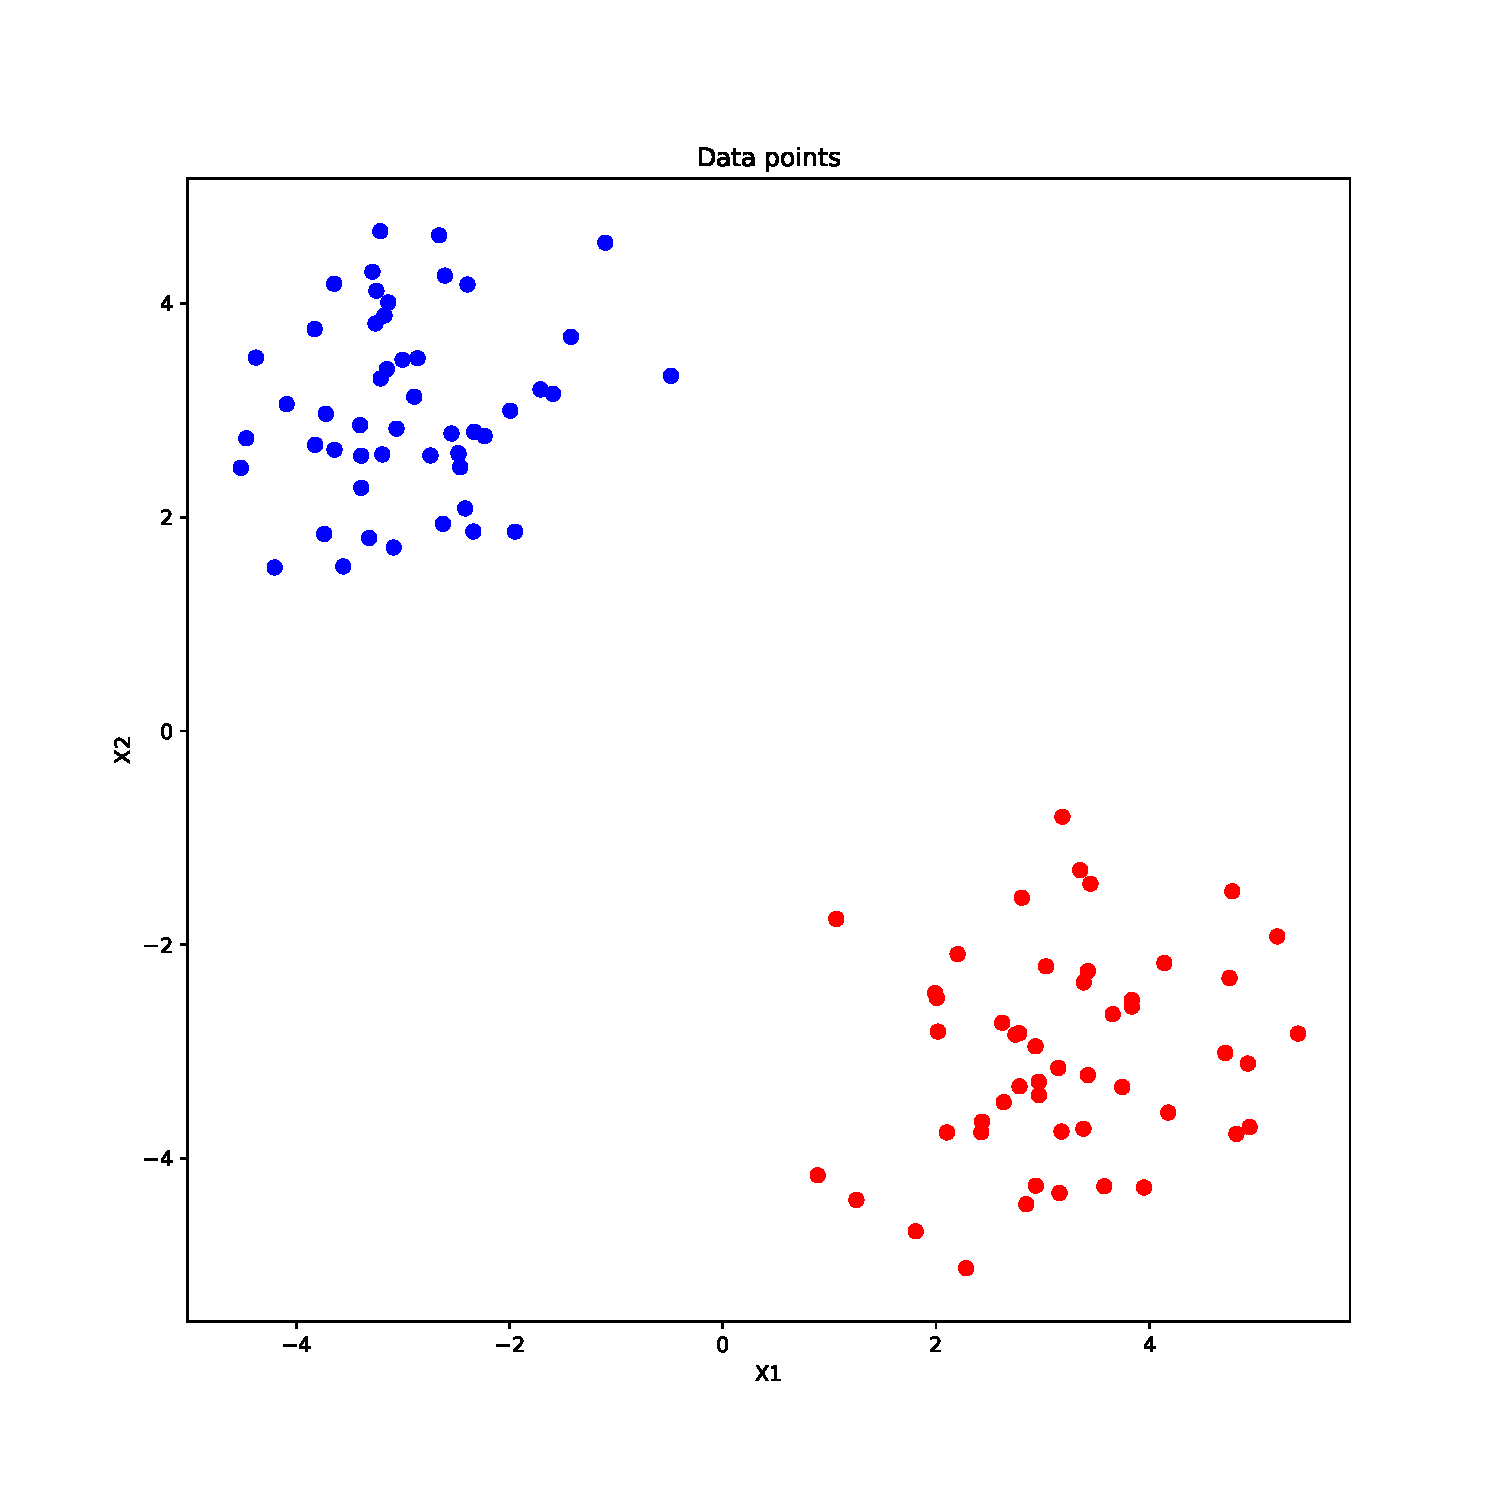
\includegraphics[width=.6\textwidth]{./Figures/1_data}
\caption{Dataset}
\label{1_1_c_mse}
\end{figure}

\begin{figure}[!ht]
	\makebox[\textwidth]{
	\begin{subfigure}{0.6\textwidth}
	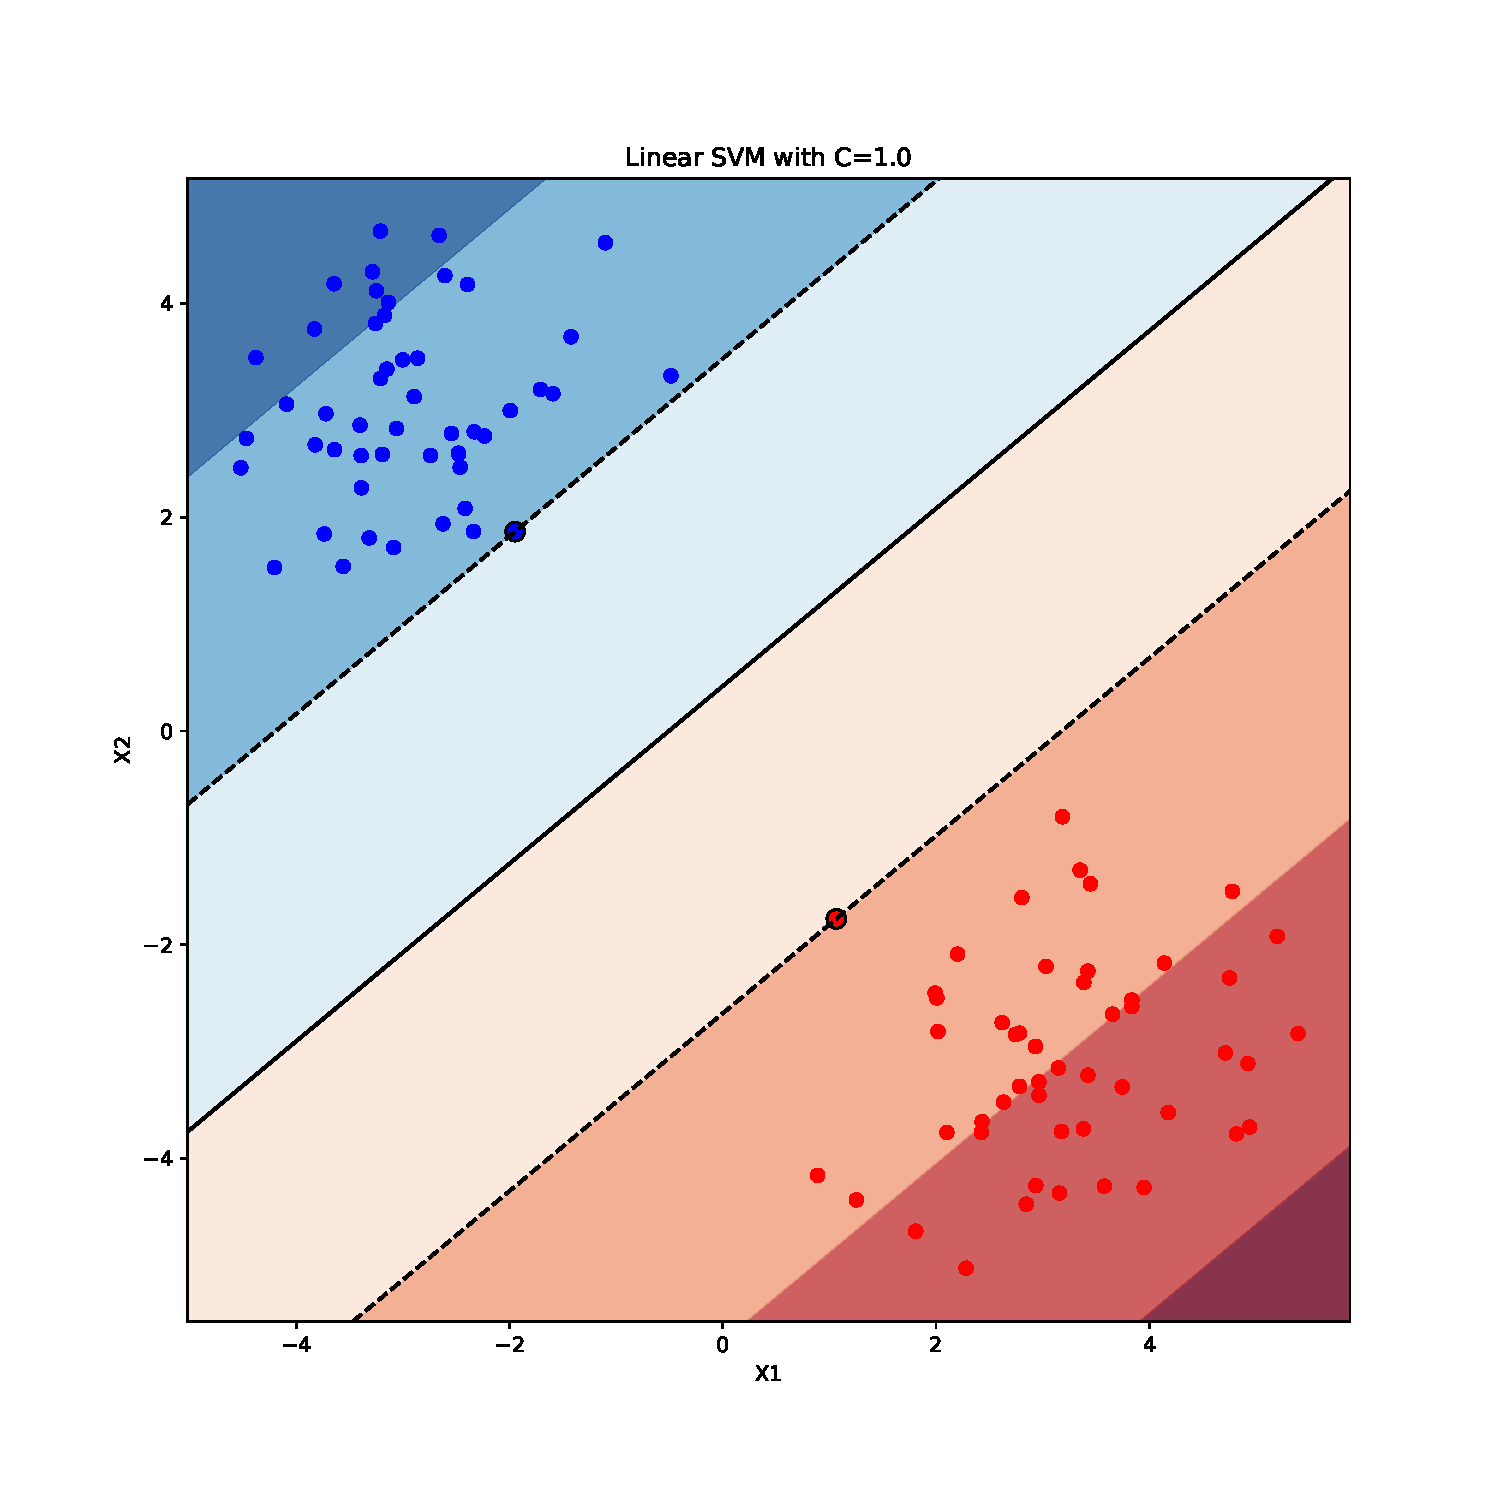
\includegraphics[width=\textwidth]{./Figures/1a_bound.pdf}
	\caption{Dataset}
	\end{subfigure}
	\begin{subfigure}{0.6\textwidth}
	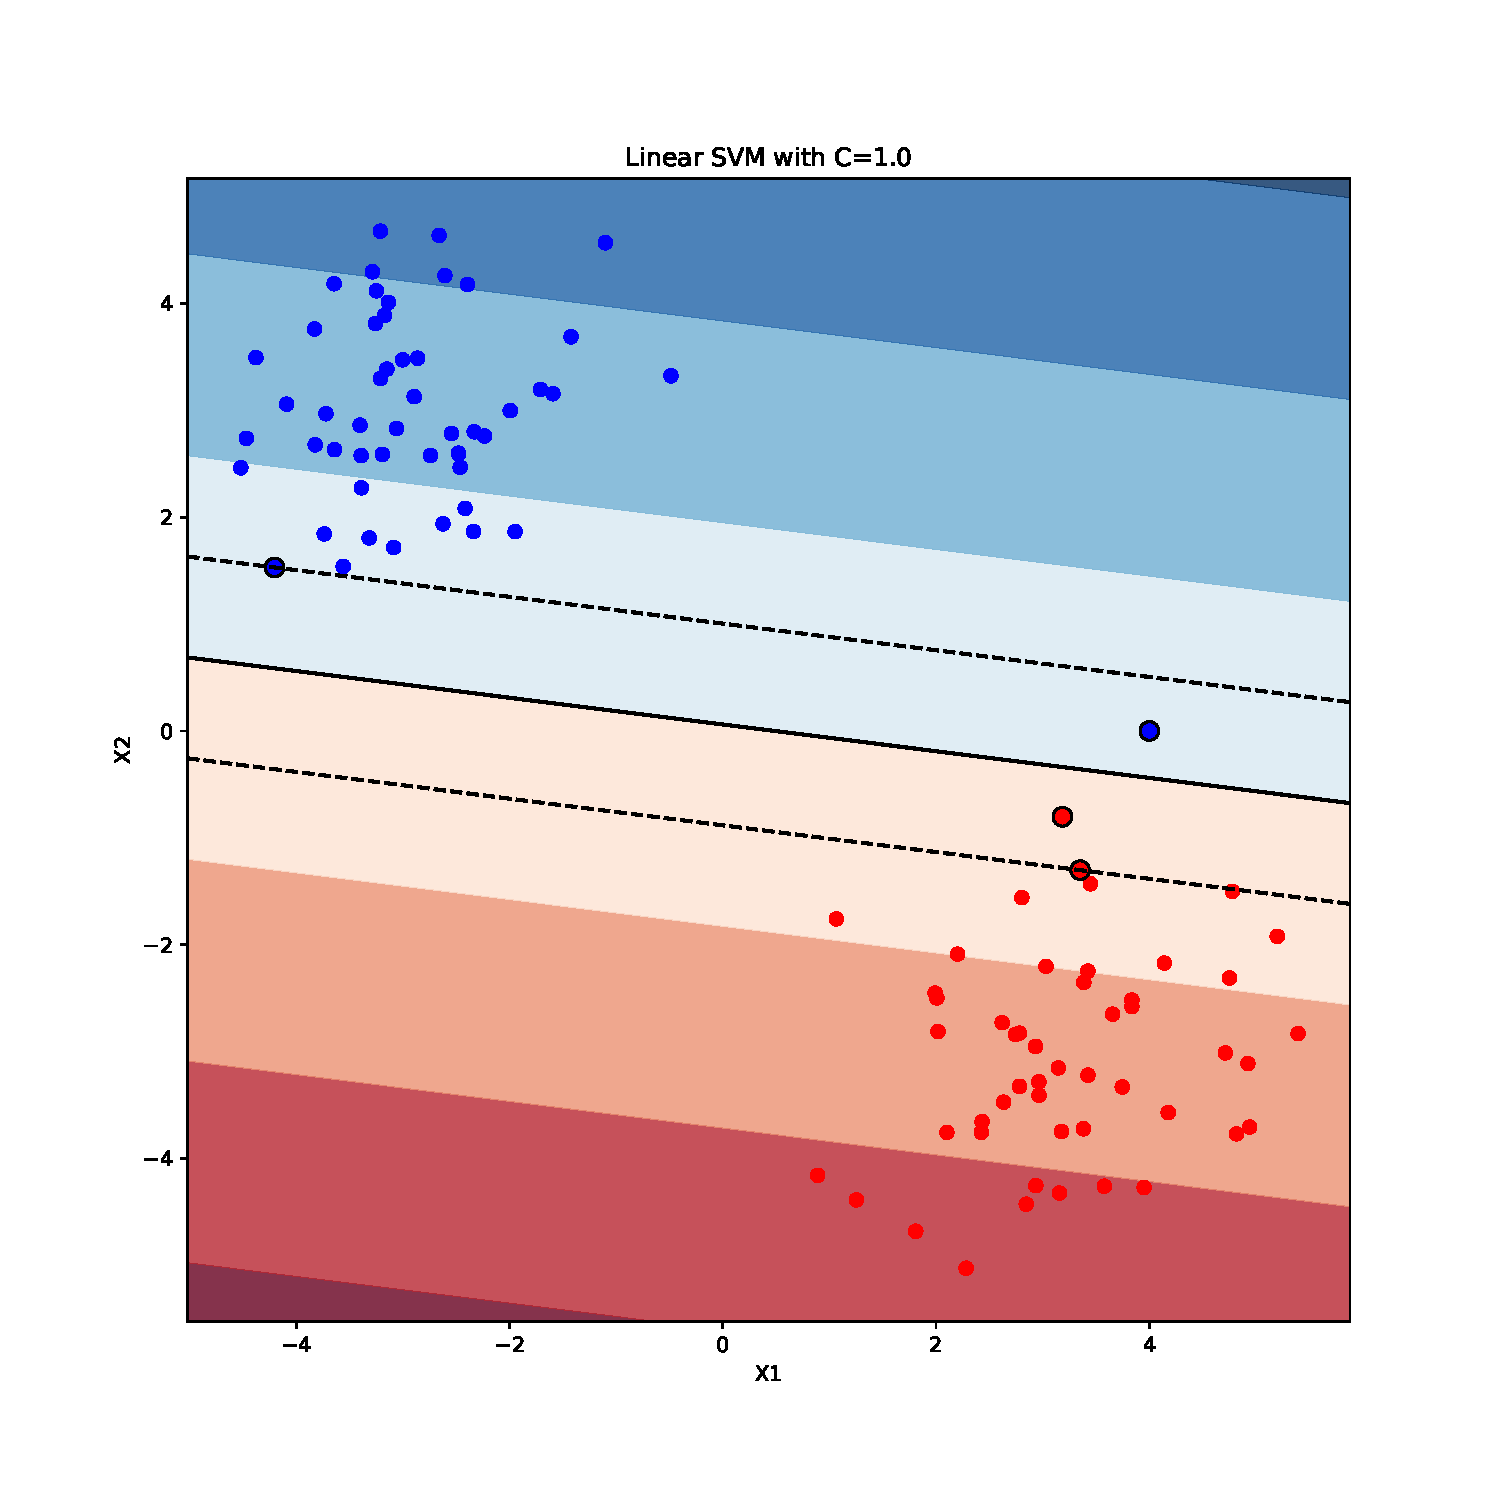
\includegraphics[width=\textwidth]{./Figures/1b_bound}
	\caption{Dataset with additional data point}
	\end{subfigure}
	}	
	\caption{Classification of the dataset using SVM}
	\label{perceptron1}
\end{figure}

\begin{figure}[!ht]
    \centering
    \makebox[\textwidth]{
    \begin{subfigure}{0.6\textwidth}
    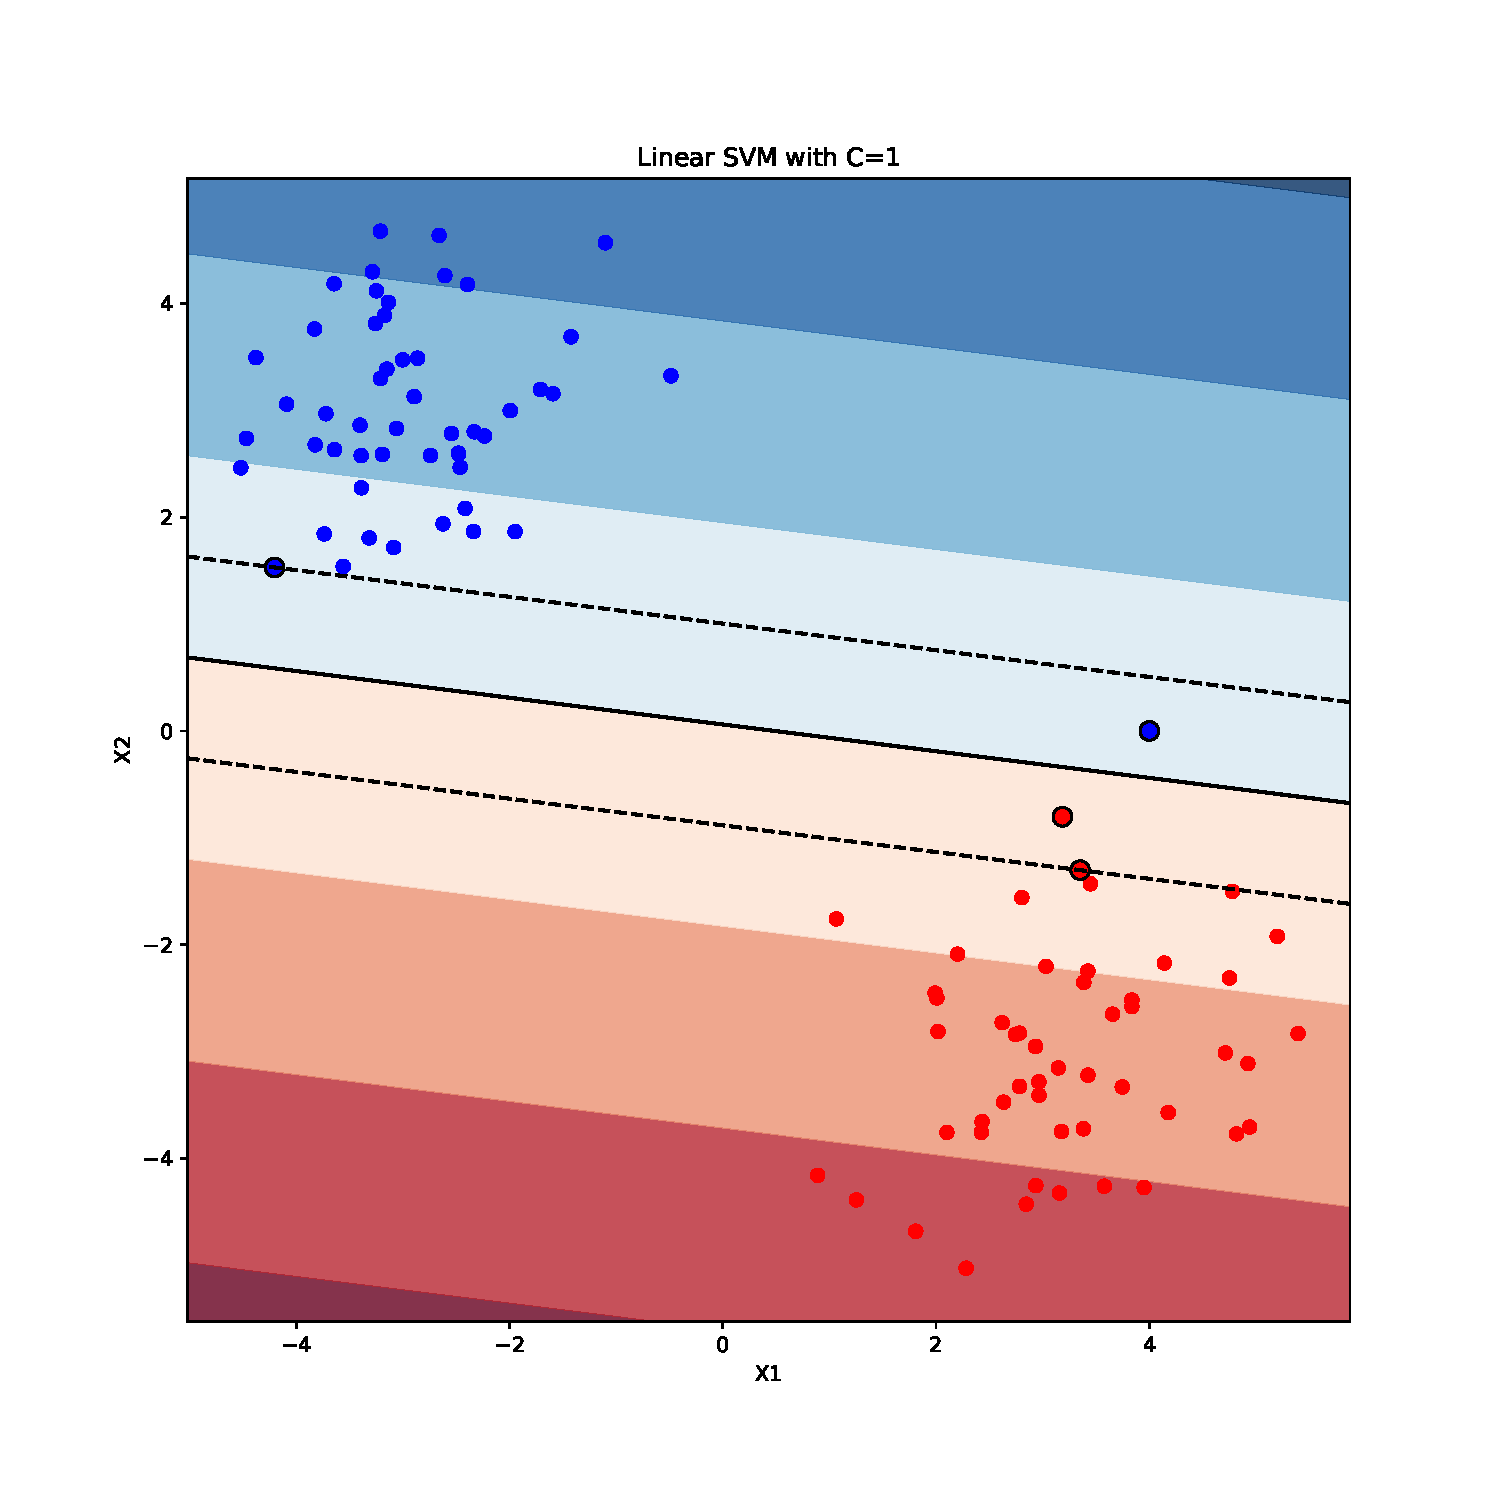
\includegraphics[width=\textwidth]{./Figures/1c_bound_C1.pdf}
    \caption{$C=1$}
    \end{subfigure}
    \begin{subfigure}{0.6\textwidth}
    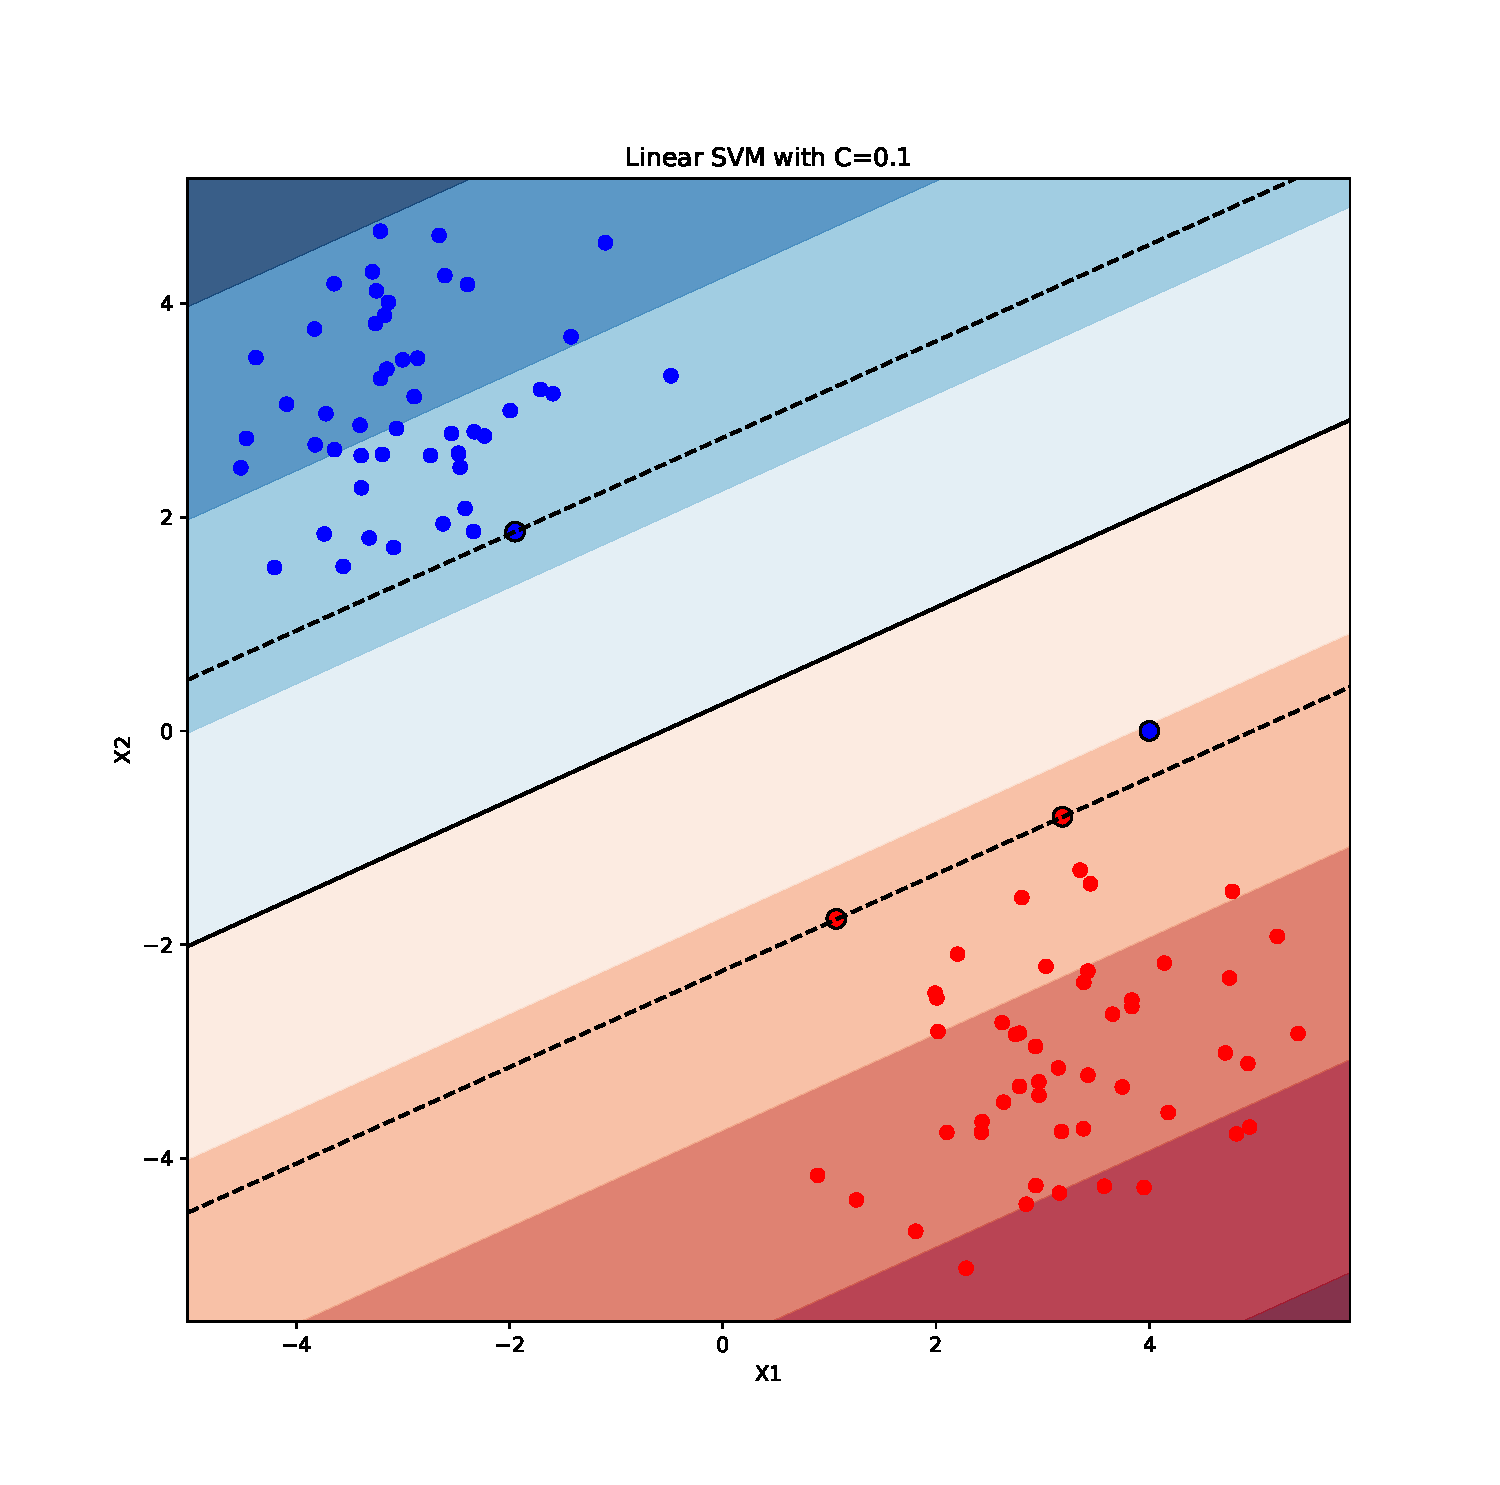
\includegraphics[width=\textwidth]{./Figures/1c_bound_C01.pdf}
    \caption{$C=0,1$}
    \end{subfigure}
    }
    
    \makebox[\textwidth]{
    \begin{subfigure}{0.6\textwidth}
    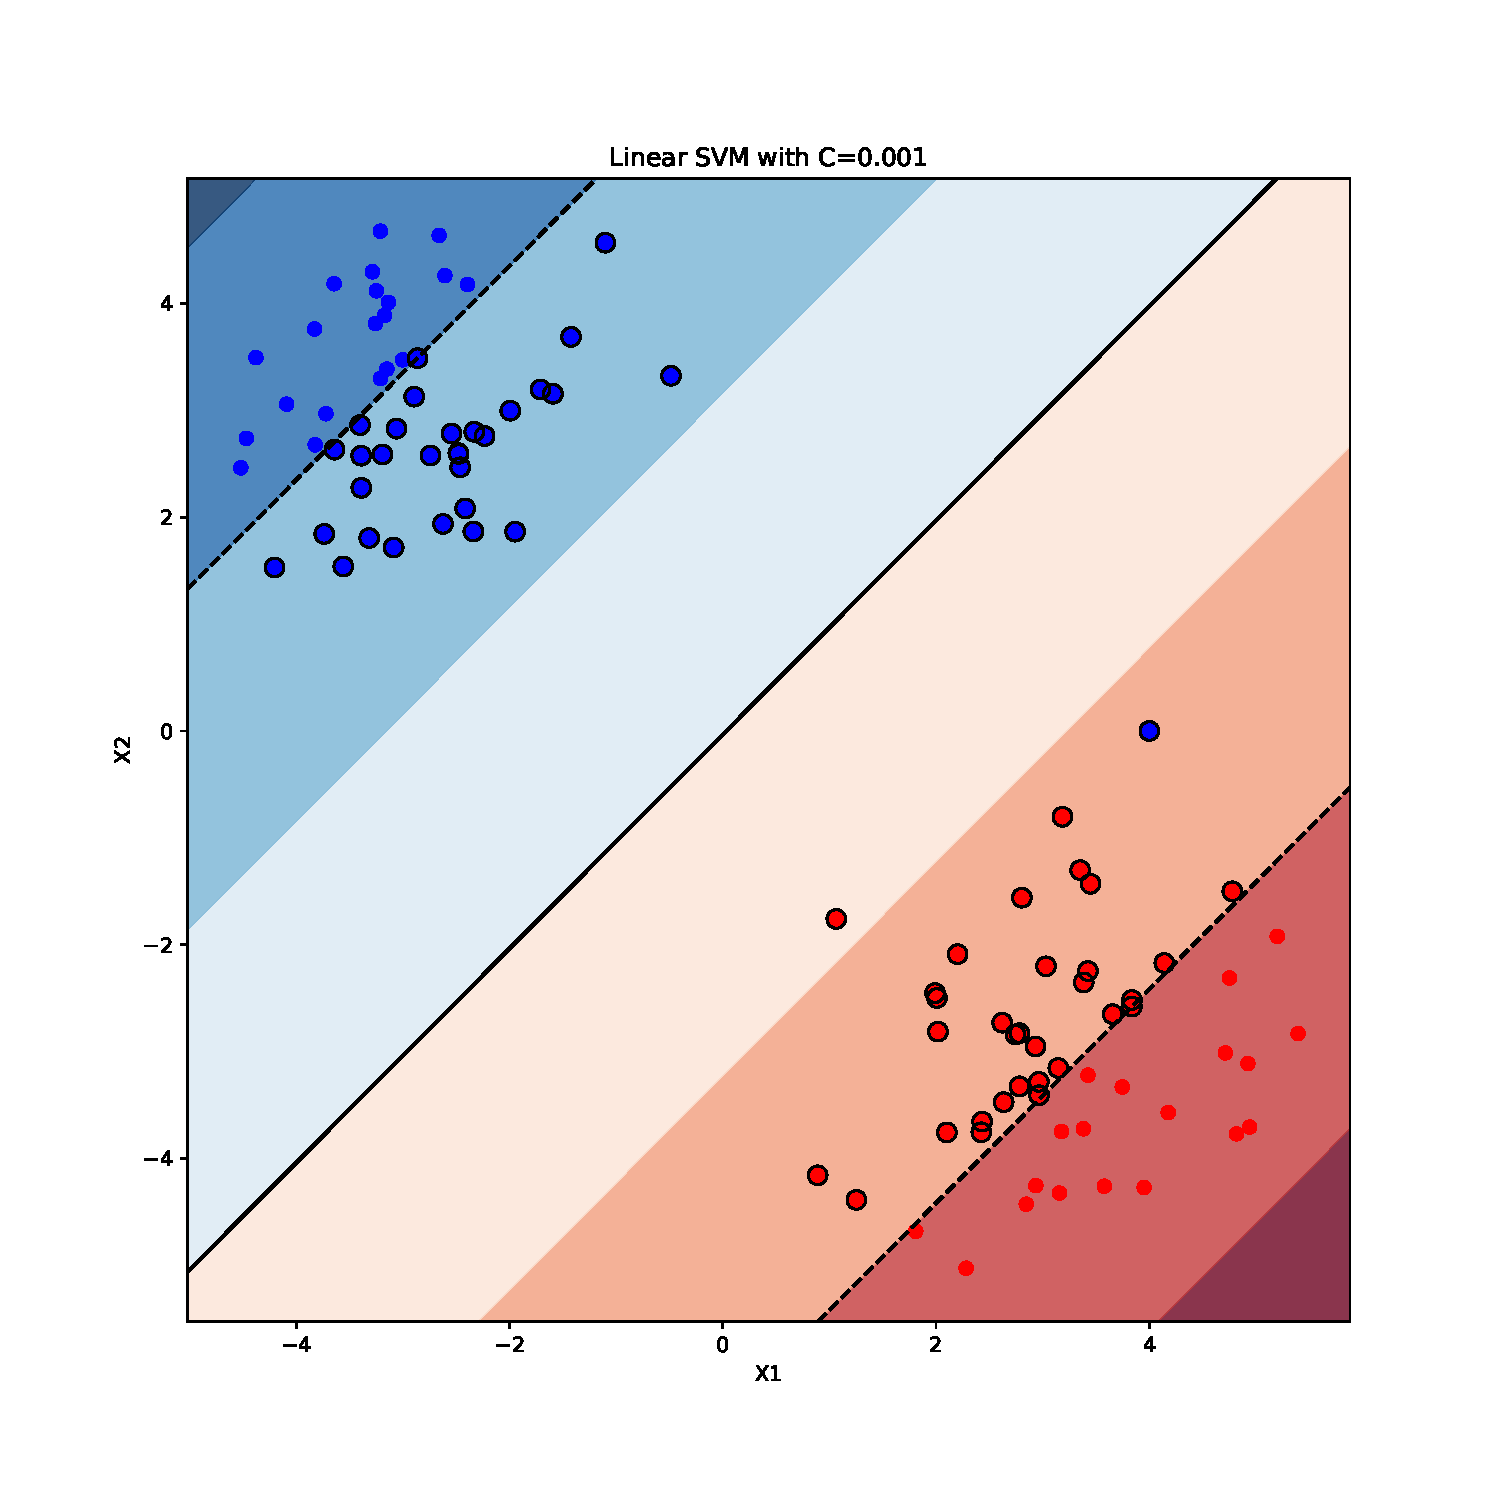
\includegraphics[width=\textwidth]{./Figures/1c_bound_C0001.pdf}
    \caption{$C=0,001$}
    \end{subfigure}
    \begin{subfigure}{0.6\textwidth}
    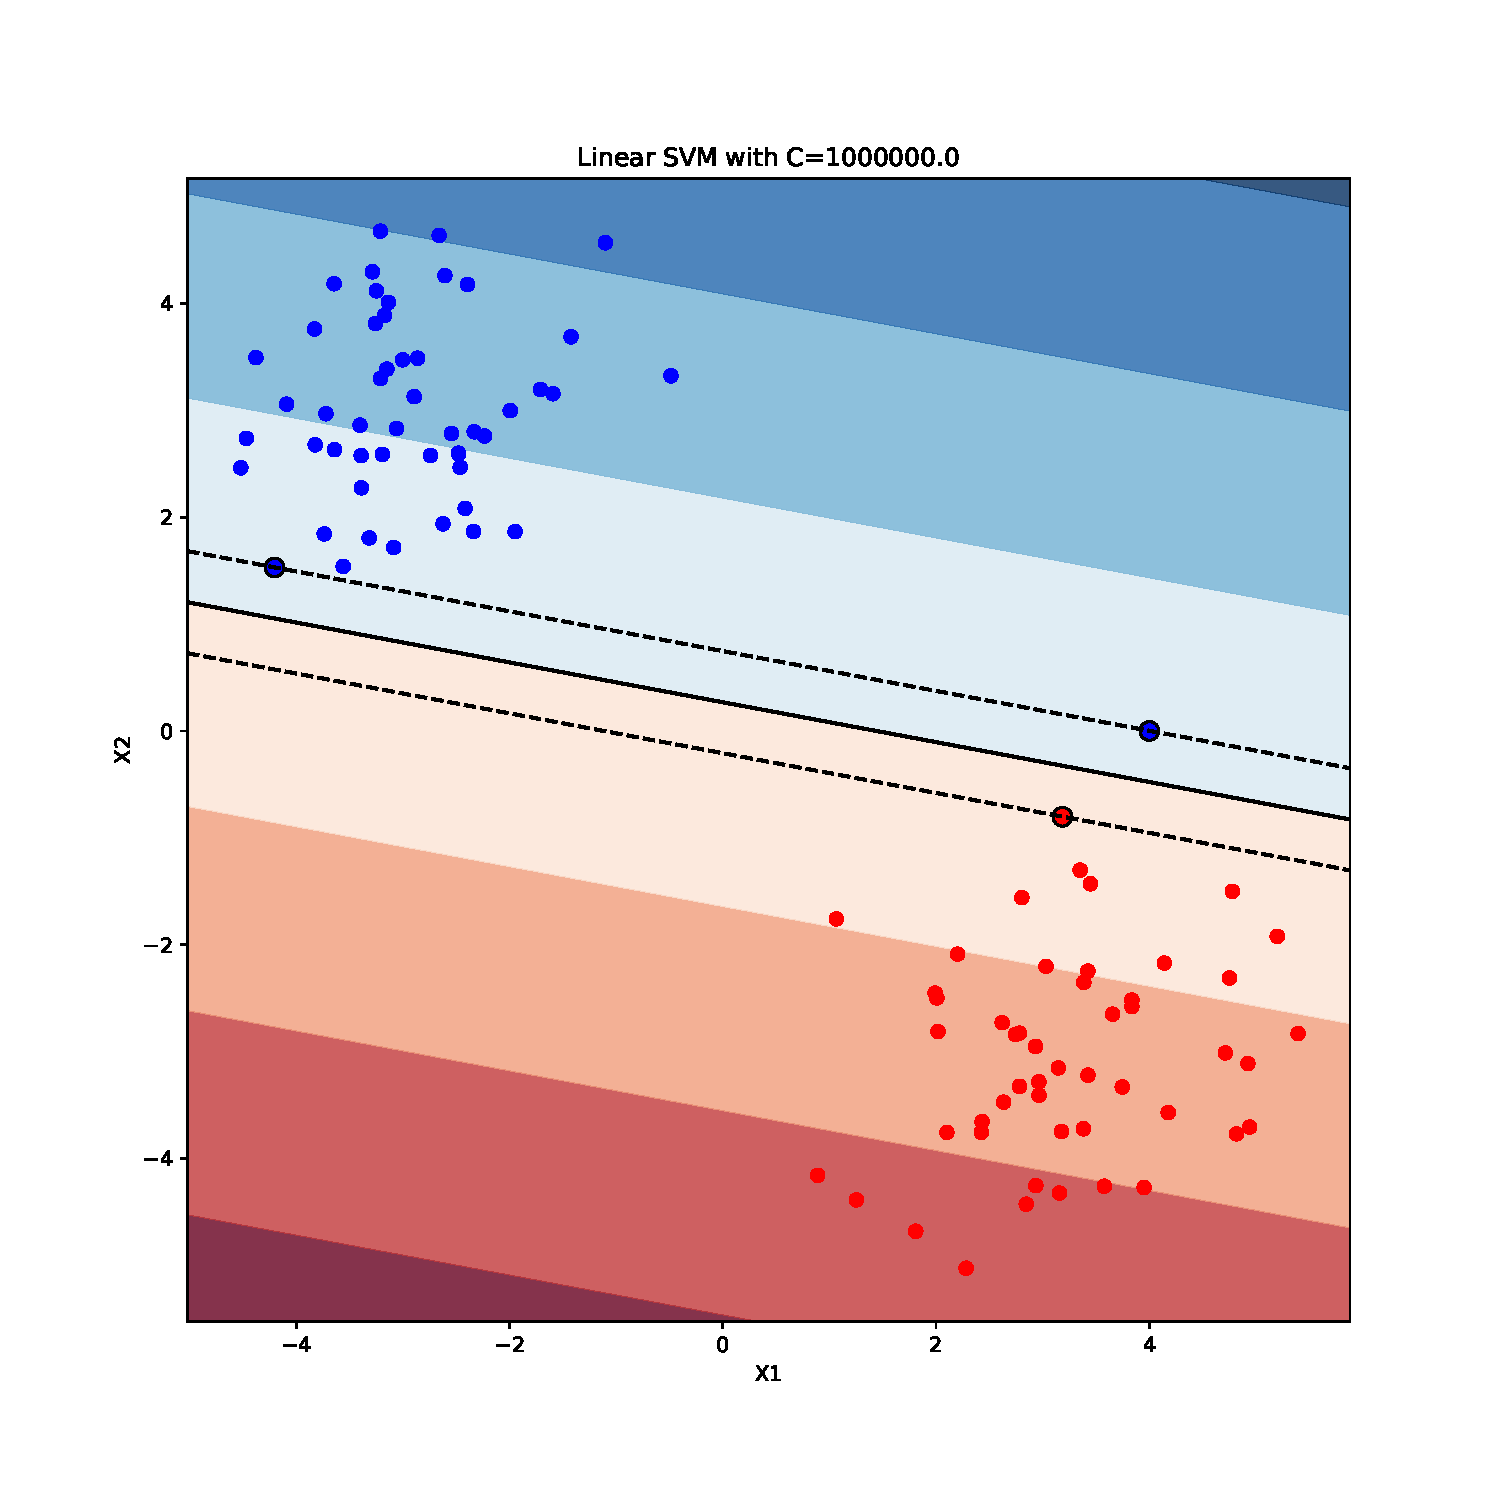
\includegraphics[width=\textwidth]{./Figures/1c_bound_C1e6.pdf}
    \caption{$C=1000000$}
    \end{subfigure}
    }
    \caption{SVM Classification using different C parameters}
    \label{misclassified_items}
\end{figure}

\subsection{How and why changed the decision boundary when the new point was added?}

The margin is defined as the perpendicular distance between the decision boundary and the closest data point. Since the new added data point is located in the margin. The algorithm adjusts its solution by choosing the option with the smallest generalization error. Apparently this includes penalized data points inside of the margin

\subsection{The inverse regularization parameter C}


\section{Nonlinear (kernel) SVM}

\subsection{}

\subsection{}

\subsection{}

\subsection{}

\subsection{}


\section{Multiclass classification}

\subsection{}

\subsection{}

\subsection{}

\subsection{}


\section{SVM with Gradient Descent}

\subsection{}

\subsection{}

\subsection{}

\subsection{}

\end{document}}